\documentclass{ximera}

\newcommand{\RR}{\mathbb R}
\renewcommand{\d}{\,d}
\newcommand{\dd}[2][]{\frac{d #1}{d #2}}
\renewcommand{\l}{\ell}
\newcommand{\ddx}{\frac{d}{dx}}
\newcommand{\dfn}{\textbf}
\newcommand{\eval}[1]{\bigg[ #1 \bigg]}


\begin{document}

\section{The shoelace algorithm}

Green's theorem can also be used to derive a simple (yet powerful!)
algorithm (often called the ``shoelace'' algorithm) for computing
areas. Here's the idea: Suppose you have a two-dimensional polygon,
where the vertices are identified by their $(x,y)$-coordinates:
\begin{image}
  \begin{tikzpicture}
    \begin{axis}%
      [
	ymin=0,ymax=12,
	xmin=0,xmax=16,
        axis lines=none,
        clip=false
      ]
      
      \addplot[penColor,ultra thick] coordinates{
        (6,11) (4,10) (2,6) (3,3) (8,2) (14,5) (9,6) (14,8) (12,10) (8,7)
      };

       \addplot[penColor!50!white,dashed,ultra thick] coordinates{
        (6,11) (8,7)
       };
      
       \addplot[color=penColor,fill=penColor,only marks,mark=*] coordinates{(6,11)};  %% closed hole
       \addplot[color=penColor,fill=penColor,only marks,mark=*] coordinates{(4,10)};  %% closed hole
       \addplot[color=penColor,fill=penColor,only marks,mark=*] coordinates{(2,6)};  %% closed hole
       \addplot[color=penColor,fill=penColor,only marks,mark=*] coordinates{(3,3)};  %% closed hole
       \addplot[color=penColor,fill=penColor,only marks,mark=*] coordinates{(8,2)};  %% closed hole
       \addplot[color=penColor,fill=penColor,only marks,mark=*] coordinates{(14,5)};  %% closed hole
       \addplot[color=penColor,fill=penColor,only marks,mark=*] coordinates{(9,6)};  %% closed hole
       \addplot[color=penColor,fill=penColor,only marks,mark=*] coordinates{(14,8)};  %% closed hole
       \addplot[color=penColor,fill=penColor,only marks,mark=*] coordinates{(12,10)};  %% closed hole
       \addplot[color=penColor,fill=penColor,only marks,mark=*] coordinates{(8,7)};  %% closed hole
       
       \node[penColor, left] at (axis cs: 4,10) {$(x_1,y_1)$};
       \node[penColor, left] at (axis cs: 2, 6) {$(x_2,y_2)$};
       \node[penColor,below left] at (axis cs: 3, 3) {$(x_3,y_3)$};
       \node[penColor,below] at (axis cs: 8, 2) {$(x_4,y_4)$};
       \node[penColor,right] at (axis cs:14, 5) {$(x_5,y_5)$};
       \node[penColor, left] at (axis cs: 9, 6) {$(x_6,y_6)$};
       \node[penColor,right] at (axis cs:14, 8) {$(x_7,y_7)$};
       \node[penColor,right] at (axis cs:12,10) {$(x_8,y_8)$};
       \node[penColor, left] at (axis cs: 8, 7) {$(x_9,y_9)$};
       \node[penColor,right] at (axis cs: 6,11) {$(x_n,y_n)$};
    \end{axis}
  \end{tikzpicture}
\end{image}
Here we see a polygon with $n$ vertices, and the ``dashed-line''
means that there could be more to this polygon than ``meets the
eye.'' So to compute the area, here is a neat trick. Write all of
the coordinates in a column, writing the starting coordinate
\textit{twice}, both at the beginning and at the end:

\begin{image}[.5in]
  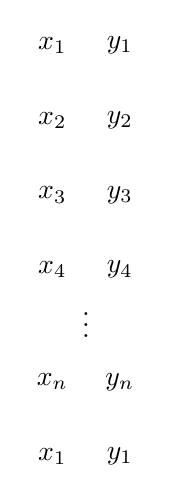
\begin{tikzpicture}
    \begin{axis}%
      [
	ymin=0,ymax=12,
	xmin=0,xmax=16,
        axis lines=none,
        clip=false
      ]      
      \node at (axis cs:0,12) {$x_1$};
      \node at (axis cs:2,12) {$y_1$};
      
      \node at (axis cs:0,10) {$x_2$};
      \node at (axis cs:2,10) {$y_2$};
      
      \node at (axis cs:0, 8) {$x_3$};
      \node at (axis cs:2, 8) {$y_3$};
      
      \node at (axis cs:0, 6) {$x_4$};
      \node at (axis cs:2, 6) {$y_4$};

      \node at (axis cs:1, 4.75) {$\vdots$};
      
      \node at (axis cs:0, 3) {$x_n$};
      \node at (axis cs:2, 3) {$y_n$};
      
      \node at (axis cs:0, 1) {$x_1$};
      \node at (axis cs:2, 1) {$y_1$};
    \end{axis}
  \end{tikzpicture}
\end{image}

Now multiply entries of the columns diagonally down from the left to the right and add them together

\begin{image}[.5in]
  \begin{tikzpicture}
    \begin{axis}%
      [
	ymin=0,ymax=12,
	xmin=0,xmax=16,
        axis lines=none,
        clip=false
      ]      
      \node at (axis cs:0,12) {$x_1$};
      \node at (axis cs:2,12) {$y_1$};

      \addplot[->,ultra thick,penColor,shorten >=0.2cm,shorten <=.2cm,] coordinates{(0,12) (2,10)};
      
      \node at (axis cs:0,10) {$x_2$};
      \node at (axis cs:2,10) {$y_2$};

      \addplot[->,ultra thick,penColor,shorten >=0.2cm,shorten <=.2cm,] coordinates{(0,10) (2,8)};
      
      \node at (axis cs:0, 8) {$x_3$};
      \node at (axis cs:2, 8) {$y_3$};

      \addplot[->,ultra thick,penColor,shorten >=0.2cm,shorten <=.2cm,] coordinates{(0,8) (2,6)};
      
      \node at (axis cs:0, 6) {$x_4$};
      \node at (axis cs:2, 6) {$y_4$};

      %\addplot[->,ultra thick,penColor,shorten >=0.2cm,shorten <=.2cm,] coordinates{(0,6) (2,4)};

      \node at (axis cs:1, 4.75) {$\vdots$};

      %\addplot[->,ultra thick,penColor,shorten >=0.2cm,shorten <=.2cm,] coordinates{(0,5) (2,3)};
      
      \node at (axis cs:0, 3) {$x_n$};
      \node at (axis cs:2, 3) {$y_n$};

      \addplot[->,ultra thick,penColor,shorten >=0.2cm,shorten <=.2cm,] coordinates{(0,3) (2,1)};
      
      \node at (axis cs:0, 1) {$x_1$};
      \node at (axis cs:2, 1) {$y_1$};
    \end{axis}
  \end{tikzpicture}
\end{image}
to obtain:
\[
x_1y_2 + x_2y_3 + x_3y_4 + \dots + x_ny_1
\]
Now, multiply entries of the columns diagonally down from the left to
the right and subtract them from our previous sum
\begin{image}[.5in]
  \begin{tikzpicture}
    \begin{axis}%
      [
	ymin=0,ymax=12,
	xmin=0,xmax=16,
        axis lines=none,
        clip=false
      ]      
      \node at (axis cs:0,12) {$x_1$};
      \node at (axis cs:2,12) {$y_1$};

      \addplot[->,ultra thick,penColor!50!white,shorten >=0.2cm,shorten <=.2cm,] coordinates{(0,12) (2,10)};
      \addplot[->,ultra thick,penColor2,shorten >=0.2cm,shorten <=.2cm,] coordinates{(2,12) (0,10)};
      
      \node at (axis cs:0,10) {$x_2$};
      \node at (axis cs:2,10) {$y_2$};

      \addplot[->,ultra thick,penColor!50!white,shorten >=0.2cm,shorten <=.2cm,] coordinates{(0,10) (2,8)};
      \addplot[->,ultra thick,penColor2,shorten >=0.2cm,shorten <=.2cm,] coordinates{(2,10) (0,8)};
      
      \node at (axis cs:0, 8) {$x_3$};
      \node at (axis cs:2, 8) {$y_3$};

      \addplot[->,ultra thick,penColor!50!white,shorten >=0.2cm,shorten <=.2cm,] coordinates{(0,8) (2,6)};
      \addplot[->,ultra thick,penColor2,shorten >=0.2cm,shorten <=.2cm,] coordinates{(2,8) (0,6)};
      
      \node at (axis cs:0, 6) {$x_4$};
      \node at (axis cs:2, 6) {$y_4$};

      %\addplot[->,ultra thick,penColor!50!white,shorten >=0.2cm,shorten <=.2cm,] coordinates{(0,6) (2,4)};

      \node at (axis cs:1, 4.75) {$\vdots$};

      %\addplot[->,ultra thick,penColor!50!white,shorten >=0.2cm,shorten <=.2cm,] coordinates{(0,5) (2,3)};
      
      \node at (axis cs:0, 3) {$x_n$};
      \node at (axis cs:2, 3) {$y_n$};

      \addplot[->,ultra thick,penColor!50!white,shorten >=0.2cm,shorten <=.2cm,] coordinates{(0,3) (2,1)};
      \addplot[->,ultra thick,penColor2,shorten >=0.2cm,shorten <=.2cm,] coordinates{(2,3) (0,1)};
      
      \node at (axis cs:0, 1) {$x_1$};
      \node at (axis cs:2, 1) {$y_1$};
    \end{axis}
  \end{tikzpicture}
\end{image}
to obtain:
\begin{align*}
  S=x_1y_2 &+ x_2y_3 + x_3y_4 + \dots + x_ny_1 \\
  &-x_2y1 - x_3y_2 - x_4y_3 - \dots - x_1y_n
\end{align*}
The area of the polygon in question will be:
\[
A = \frac{|S|}{2}
\]
The algorithm is called the ``shoelace'' algorithm because of the
crisscrossing pattern you see above.

\begin{question}
  Compute the area of the following polygon:
  %% Give some poly
  \begin{prompt}
    The area is $\answer{47}$ square units.
  \end{prompt}
\end{question}

\subsection{Why does the shoelace algorithm work?}

Now we are going explain why the shoelace algorithm works via Green's
Theorem. The restrained young mathematician may protest that we are
using a ``crane to crush a fly,'' but whatever. We like Green's
Theorem. To start, recall that if $\vec{F} = \vector{0,x}$, then $\curl\vec{F}(x,y) = 1$. Hence Green's Theorem states:
\[
\iint_R \d A = \oint_P x\d y
\]
This means we can compute the area of the region $R$, by evaluating
the line integral on the right along the polygonal boundary $P$. So again
consider a polygon whose vertices are:
\[
(x_1,y_1),(x_2,y_2),\dots,(x_n,y_n)
\]
In this case, $P$ can be broken into $n$ edges, (if a polygon has $n$ vertices, it has $n$ edges) that we can easily parameterize as
\begin{align*}
  E_1 &: \vector{x_1,y_1} + t \vector{x_2-x_1,y_2-y_1}\\
  E_2 &: \vector{x_2,y_2} + t \vector{x_3-x_2,y_3-y_2}\\
  E_3 &: \vector{x_3,y_3} + t \vector{x_4-x_3,y_4-y_3}\\
  &\vdots\\
  E_n &: \vector{x_n,y_n} + t \vector{x_n-x_1,y_n-y_1}
\end{align*}
with $0\le t<1$ in each case. Moreover
\[
\oint_P x\d y = \sum_{i=1}^n \int_{E_i} x\d y,
\]
this is just saying that the line integral along the perimeter of the polygon is the sum of the line integrals along the edges. 
\end{document}
